%---------- Inleiding ---------------------------------------------------------

\section{Introductie} % The \section*{} command stops section numbering
\label{sec:introductie}
Het correct én efficiënt verwerken van klantenaankopen is een cruciaal process binnen de retailsector. Om die reden investeert Colruyt Group momenteel in nieuwe touchscreens voor haar voornaamste kassasysteem, alsook een herwerking van de checkoutsoftware die deel uitmaakt van het systeem.

Dit systeem wordt gebruikt worden binnen de filialen van de retailformules Colruyt (België, Luxemburg, en Frankrijk), OKay en OKay City, Bio-Planet, Dreamland en Dreambaby, alsook door de zelfstandige ondernemers van Spar.

Hoewel de ontwikkeling van deze software met rasse schreden vooruit gaat, werd er tot op heden maar weinig geïnvesteerd in (geautomatiseerde) e2e\footnote{\textbf{End to end (e2e) testing} — Een techniek binnen software testing waarbij alle componenten van het systeem getest worden middels het simuleren van werkelijke geburikersscenario's ~\cite{SoftwareTestingHelp2019}.}. Nochtans is de stabiliteit van het kassasysteem een onbetwistbare noodzaak voor groep.

Bovendien wordt de software continu uitgebreid met nieuwe functionaliteit en moet het probleemloos kunnen interfacen met een waslijst aan andere systemen (barcodelezers, weegschalen, betaalterminals, de systemen van stockbeheer, productinformatie, finance, customer relations, marketing \& promotie etc.).
\vspace{\baselineskip}
Een robuust testsysteem is bijgevolg onontbeerlijk en ondersteunt de softwareontwikkeling door:

\begin{itemize}
  \item het vroegtijdig onderscheppen van defecten
  \item een grotere test coverage
  \item een grotere efficiëntie van testen
  \item een snellere time-to-market
  \item een verlaging van de ontwikkelingskosten
\end{itemize}

De eerste stap voor het uitbouwen van een testsysteem is het kiezen van een gepast testing framework. Ook voor een relatief jong framework zoals Angular zijn er reeds verschillende alternatieven beschikbaar.
\vspace{\baselineskip}
Het onderzoek dat onderwerp is van dit voorstel bestaat er dus uit om na te gaan:

\begin{itemize}
    \item welke e2e testing frameworks bestaan voor Angular en welke randvoorwaarden (kost, beschikbare ondersteuning en documentatie, vereiste programmeervaardigheden) zij hebben,
    \item in welke mate de bestaande frameworks de volledige functionaliteit van het systeem kunnen afdekken,
    \item hoe performant elk van de frameworks is en
    \item hoe betrouwbaar de resultaten van de frameworks zijn
\end{itemize}

om zo het meest geschikte framework voor de use case van Colruyt Group te kunnen aanbevelen.

%---------- Stand van zaken ---------------------------------------------------

\section{State-of-the-art}
\label{sec:state-of-the-art}

De keuze voor een geschikt e2e testing framework is sterk afhankelijk van de specifieke context waarbinnen dit gebruikt gaat worden. Colruyt Group overweegt momenteel 2 verschillende frameworks:

\begin{itemize}
    \item \textbf{Protractor} — een API voor e2e testing die steunt op Selenium (een ``WebDriver'' die webapplicaties voor testdoeleinden automatiseert)
    \item \textbf{Cypress} — een relatief nieuw e2e framework
\end{itemize}

\vspace{\baselineskip}

Daarnaast zijn er nog een reeks andere Behavior-Driven Development of testing frameworks voor het JavaScript ecosysteem. De meest prominente frameworks die van toepassing zijn op Angular, buiten bovenstaande, zijn de volgende:

\begin{itemize}
    \item \textbf{Jasmine}
    \item \textbf{Jest}
    \item \textbf{Mocha}
    \item \textbf{Puppeteer}
    \item \textbf{AVA}
    \item \textbf{Cucumber}
\end{itemize}

\vspace{\baselineskip}

Zie ook ~\cite{Castro2019}; ~\cite{Definition2019}; ~\cite{Kamalizade2019}; ~\cite{Lotanna2019}; ~\cite{Roy2019} en ~\cite{Zaidman2019}.

%Hier beschrijf je de \emph{state-of-the-art} rondom je gekozen onderzoeksdomein. Dit kan bijvoorbeeld een literatuurstudie zijn. Je mag de titel van deze sectie ook aanpassen (literatuurstudie, stand van zaken, enz.). Zijn er al gelijkaardige onderzoeken gevoerd? Wat concluderen ze? Wat is het verschil met jouw onderzoek? Wat is de relevantie met jouw onderzoek?

%Verwijs bij elke introductie van een term of bewering over het domein naar de vakliteratuur, bijvoorbeeld~\autocite{Doll1954}! Denk zeker goed na welke werken je refereert en waarom.

% Voor literatuurverwijzingen zijn er twee belangrijke commando's:
% \autocite{KEY} => (Auteur, jaartal) Gebruik dit als de naam van de auteur
%   geen onderdeel is van de zin.
% \textcite{KEY} => Auteur (jaartal)  Gebruik dit als de auteursnaam wel een
%   functie heeft in de zin (bv. ``Uit onderzoek door Doll & Hill (1954) bleek
%   ...'')

%Je mag gerust gebruik maken van subsecties in dit onderdeel.

%---------- Methodologie ------------------------------------------------------
\section{Methodologie}
\label{sec:methodologie}

Om het meest geschikte framework voor Colruyt Group's checkoutsysteem te kunnen identificeren, dienen volgende stappen genomen te worden:

\begin{enumerate}
    \item onderzoek naar de \textbf{mogelijkheden en randvoorwaarden} van elke kandidaat, om daar de 3 meest geschikte kandidaten uit te halen
    \item onderzoek naar de \textbf{huidige functionaliteit} van het kassasysteem, alsook de bestaande interfacing met randapparaten en andere systemen
    \item de selectie van een \textbf{representatieve subset} van de functionaliteit van het kassasysteem
    \item schrijven van \textbf{identieke testscenario's} in elk van de 3 gekozen testing frameworks
    \item opzetten van de frameworks, \textbf{uitvoeren van de testscenario's} en meten van de performantie (complexiteit van installatie, benodigde tijd om testen te schrijven, doorlooptijd, geheugengebruik)
    \item formuleren van een \textbf{advies} op basis van de gegevens verzameld in de voorgaande stappen
\end{enumerate}
\vspace{\baselineskip}
Dit advies is het eindresultaat van dit onderzoek.

%Hier beschrijf je hoe je van plan bent het onderzoek te voeren. Welke onderzoekstechniek ga je toepassen om elk van je onderzoeksvragen te beantwoorden? Gebruik je hiervoor experimenten, vragenlijsten, simulaties? Je beschrijft ook al welke tools je denkt hiervoor te gebruiken of te ontwikkelen.

%---------- Verwachte resultaten ----------------------------------------------
\section{Verwachte resultaten}
\label{sec:verwachte_resultaten}

De resultaten voor dit onderzoek zijn moeilijk te anticiperen omwille van het veelvoud aan variabelen die van toepassing zijn. Elk van de verschillende testingframeworks zal vermoedelijk voor- en nadelen hebben en het uiteindelijke advies zal afhangen van de specifieke behoeften van Colruyt Group en de eigenschappen van het Checkoutsysteem.

Naast een overzicht van de mogelijkheden en randvoorwaarden van elk testing framework, zullen de resultaten van de testscenario's een objectief beeld van de voor- en nadelen van elk framework kunnen geven.

    \begin{figure}[h!]
    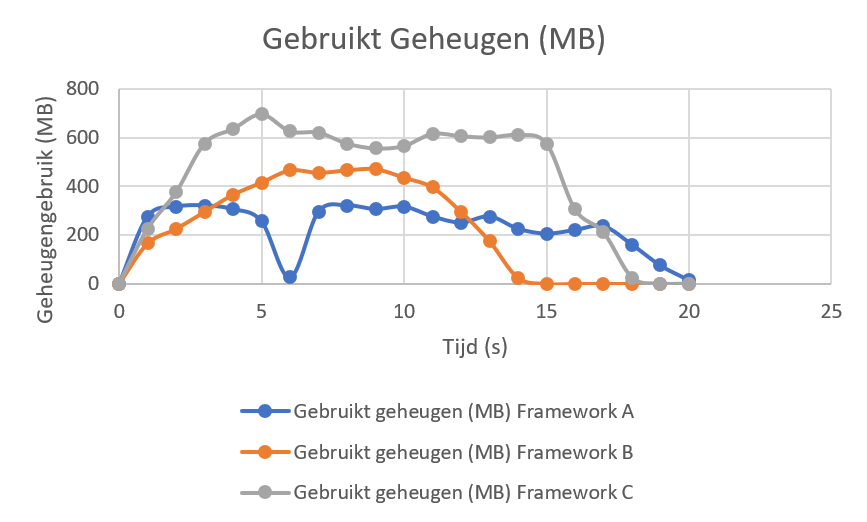
\includegraphics[width=\linewidth]{img/gebruiktgeheugen.PNG}
    \caption{Mock grafiek: Geheugengebruik in MB van de verschillende testframeworks tijdens het uitvoeren van de testscenario's.}
    \label{fig:geheugenmock}
    \end{figure}

    \begin{figure}[h!]
    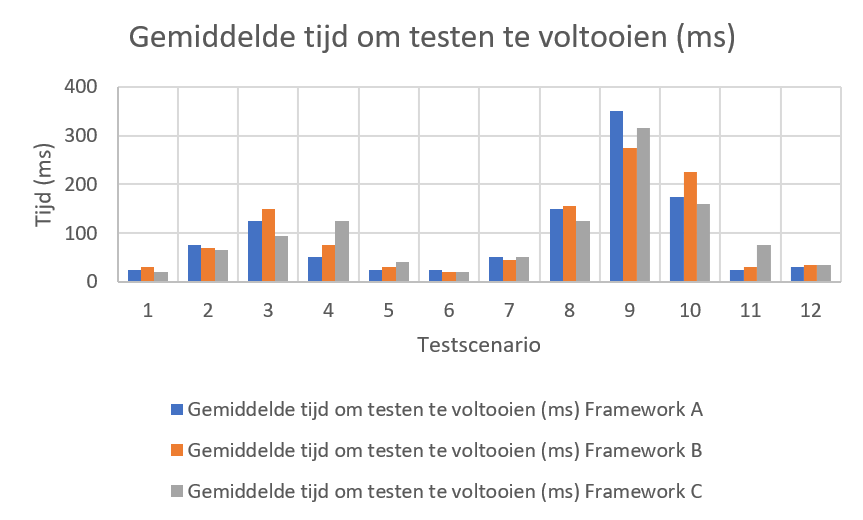
\includegraphics[width=\linewidth]{img/gemtijdtestenvoltooien.PNG}
    \caption{Mock grafiek: Benodigde tijd om elk van de verschillende testscenario's uit te voeren.}
    \label{fig:uitvoertijdmock}
    \end{figure}

%Hier beschrijf je welke resultaten je verwacht. Als je metingen en simulaties uitvoert, kan je hier al mock-ups maken van de grafieken samen met de verwachte conclusies. Benoem zeker al je assen en de stukken van de grafiek die je gaat gebruiken. Dit zorgt ervoor dat je concreet weet hoe je je data gaat moeten structureren.

%---------- Verwachte conclusies ----------------------------------------------
\section{Verwachte conclusies}
\label{sec:verwachte_conclusies}

Zoals reeds eerder vermeld, is het moeilijk om in te schatten welk framework uiteindelijk geadviseerd zal worden. De ontwikkelaars van het checkoutsysteem lijken in eerste instantie de voorkeur te geven aan het recentere Cypress, vooral omdat testen schrijven in dit framework intuïtiever en sneller zou zijn. In welke mate een framework aanvaard wordt is vaak de doorslaggevende factor om een bepaald framework te kiezen, en het lijkt dus aannemelijk dat Cypress uiteindelijk opgenomen wordt in het advies.

%Hier beschrijf je wat je verwacht uit je onderzoek, met de motivatie waarom. Het is \textbf{niet} erg indien uit je onderzoek andere resultaten en conclusies vloeien dan dat je hier beschrijft: het is dan juist interessant om te onderzoeken waarom jouw hypothesen niet overeenkomen met de resultaten.

